% Source: Lecture7.pdf, pages 3-7 (the Potts model).
\subsection{The Potts model and its solution in one dimension}
\subsubsection*{From the Ising model to the Potts model}

Next, discuss a generalization of the Ising model. The dynamical variables in the Ising model take on 2 values,
$\sigma_i = \pm1$. The spin--spin interaction (with $H = 0$)
\begin{equation}
  \Ham_{\text{int.}}^{(I)} = -J_I\sum_{\langle ij\rangle_{\text{n.n.}}}\sigma_i\sigma_j
\end{equation}
also takes on 2 values: $-J_I$ for the pairs $++$, $--$, and $+J_I$ for the pairs $+-$, $-+$; the difference is $2|J_I|$,
where we use a superscript or subscript $I$ to denote Ising.

This is equivalent to a model in which the dynamical variables $\sigma_i$ take on the values 1 or 2 and the spin--spin
interaction involves a Kronecker $\delta_{\sigma_i\sigma_j}$:
\begin{equation}
  \Ham_{\text{int.}}^{(P)} = -J_P\sum_{\langle ij\rangle_{\text{n.n.}}}\delta_{\sigma_i\sigma_j}\qquad(H = 0),
\end{equation}
with $\Ham_{\text{int.}} = -J_P$ for the pairs $11$, $22$ and $\Ham_{\text{int.}} = 0$ for the pairs $12$, $21$; the difference
is $|J_P|$. If $J>0$, $\Ham_{\text{int.}}$ prefers $\sigma_i$ and $\sigma_j$ to have the same value. If $J<0$,
$\Ham_{\text{int.}}$ prefers $\sigma_i$ and $\sigma_j$ to have different values. These formulations are equivalent if we set
$2J_I = J_P$ and shift the zero of the energy by a constant. This constant $c$ divides out in any thermal average, since
\begin{equation}
  \ev{\mathcal O} = \frac{\sum_{\text{states}}\mathcal Oe^{-\beta(\Ham+c)}}{\sum_{\text{states}}e^{-\beta(\Ham+c)}}
  = \frac{\sum_{\text{states}}\mathcal Oe^{-\beta\Ham}}{\sum_{\text{states}}e^{-\beta\Ham}}.
\end{equation}

Now we can generalize this model further; we let each dynamical variable $\sigma_i$ take on $q$ values:
$\sigma_i\in\{1,2,\ldots,q\}$. This is the $q$-state Potts model, and we have shown the equivalence of the 2-state Potts
model with the Ising model.

\subsubsection*{Transfer-matrix solution of the 1D Potts model}

We can use a transfer-matrix method inductively to solve for the free energy of the $q$-state Potts model on a 1D lattice.
Again, we assume PBC (and take zero external field for this calculation). Then
\begin{equation}
  Z = \sum_{\{\sigma_i\}}e^{-\beta\Ham} = \sum_{\{\sigma_i\}}e^{K_P\sum_{\langle ij\rangle}\delta_{\sigma_i\sigma_j}} = \Tr(T^N),
  \qquad K_P\equiv\beta J_P,
\end{equation}
where $T$ is the transfer matrix, with matrix elements
\begin{equation}
  \langle\sigma_i|T|\sigma_j\rangle = e^{K_P\delta_{\sigma_i\sigma_j}}
  = \begin{cases} e^{K_P} & \text{if } \sigma_i = \sigma_j\\ e^0 = 1 & \text{if } \sigma_i\ne\sigma_j .\end{cases}
\end{equation}
Let $e^{K_P}\equiv y$, and consider the first few cases.

\paragraph{Case $q = 2$.} In the basis of states $(1,2)$,
\begin{equation}
  T = \begin{pmatrix} e^{K_P} & 1\\ 1 & e^{K_P}\end{pmatrix} = \begin{pmatrix} y & 1\\ 1 & y\end{pmatrix};
\end{equation}
the indicial equation for the eigenvalues is $(y-\lambda)^2-1 = 0$, i.e.\ $\lambda^2-2\lambda y+y^2-1 = 0$
\begin{equation}
  \Rightarrow\quad\lambda = \tfrac12\left[2y\pm\sqrt{4y^2-4(y^2-1)}\right] = \tfrac12\left[2y\pm 2\right] = y\pm 1;
  \qquad\lambda_{\max} = y+1 .
\end{equation}
So
\begin{equation}
  Z = \Tr(T^N) = \Tr(T_{\text{diag}}^N) = \lambda_+^N + \lambda_-^N = (y+1)^N + (y-1)^N,
\end{equation}
and the reduced free energy in the thermodynamic limit is
\begin{equation}
  f = \lim_{N\to\infty}\frac1N\ln Z = \ln\lambda_{\max} = \ln(y+1) = \ln\left(e^{K_P}+1\right),
\end{equation}
recalling
\begin{align}
  \lim_{N\to\infty}\frac1N\ln\left\{(y+1)^N\left[1+\left(\frac{y-1}{y+1}\right)^N\right]\right\}
  &= \lim_{N\to\infty}\left\{\ln(y+1) + \frac1N\ln\left[1+\left(\frac{y-1}{y+1}\right)^N\right]\right\}\nonumber\\
  &= \ln(y+1).
\end{align}

\paragraph{Case $q = 3$.} Here, the transfer matrix takes the form, with the basis of states ordered as $(1,2,3)$,
\begin{equation}
  T = \begin{pmatrix} y & 1 & 1\\ 1 & y & 1\\ 1 & 1 & y\end{pmatrix}.
\end{equation}
The indicial equation for the eigenvalues is
\begin{equation}
  \left[\lambda-(y-1)\right]^2\left[\lambda-(y+2)\right] = 0
  \ \Rightarrow\ \text{eigenvalues: }\
  \lambda = \begin{cases} y-1, & \text{multiplicity 2}:\ \lambda_{\min}\\ y+2, & \text{multiplicity 1}:\ \lambda_{\max},\end{cases}
\end{equation}
so
\begin{equation}
  Z = \Tr(T^N) = \sum_j\lambda_j^N = \lambda_{\max}^N + 2\lambda_{\min}^N
    = \lambda_{\max}^N\left[1+2\left(\frac{\lambda_{\min}}{\lambda_{\max}}\right)^N\right],
\end{equation}
where $(\lambda_{\min}/\lambda_{\max})^N\to 0$ as $N\to\infty$, and
\begin{equation}
  f = \lim_{N\to\infty}\frac1N\ln Z = \underbrace{\ln\lambda_{\max}}_{\ln(y+2)}
    + \underbrace{\lim_{N\to\infty}\frac1N\ln\left[1+2\left(\frac{\lambda_{\min}}{\lambda_{\max}}\right)^N\right]}_{0}
    = \ln(y+2).
\end{equation}

\paragraph{Case $q = 4$.}
\begin{equation}
  T = \begin{pmatrix} y & 1 & 1 & 1\\ 1 & y & 1 & 1\\ 1 & 1 & y & 1\\ 1 & 1 & 1 & y\end{pmatrix};
\end{equation}
the equation for the eigenvalues is $\left[\lambda-(y-1)\right]^3\left[\lambda-(y+3)\right] = 0$
\begin{equation}
  \Rightarrow\quad\lambda = \begin{cases} y-1 & \text{with multiplicity 3}:\ \lambda_{\min}\\ y+3 & \text{with multiplicity 1}:\ \lambda_{\max}.\end{cases}
\end{equation}
As before, $Z = \sum_j\lambda_j^N = \lambda_{\max}^N + 3\lambda_{\min}^N$, $f = \ln\lambda_{\max} = \ln(y+3)$.

\paragraph{General $q$.} By inductive reasoning, the case of general $q$ now follows:
\begin{equation}
  T_{ij} = \begin{cases} y & \text{if } i = j\\ 1 & \text{if } i\ne j\end{cases}
  \ \Rightarrow\ \text{eigenvalue }\
  \lambda = \begin{cases} y-1, & \text{multiplicity } q-1\\ y+q-1, & \text{multiplicity } 1,\end{cases}
\end{equation}
\begin{equation}
  Z = \lambda_{\max}^N + (q-1)\lambda_{\min}^N = (y+q-1)^N + (q-1)(y-1)^N\equiv(q+v_P)^N + (q-1)v_P^N,
\end{equation}
where $v_P = y-1$, and
\begin{equation}
  f = \lim_{N\to\infty}\frac1N\ln Z = \ln(y+q-1) = \ln(q+v_P) = \ln\left(q+e^{K_P}-1\right).
\end{equation}

\paragraph{Internal energy.} The internal energy per site is, with $y = e^{K_P}\Rightarrow\frac{\dd y}{\dd K_P} = y$,
\begin{equation}
  \bar U = -\pder f\beta = -J_P\pder{f}{K_P} = -J_P\pder{y}{K_P}\pder fy
  = -J_Py\pder{}{y}\ln(y+q-1) = -J_P\left(\frac{y}{y+q-1}\right),
\end{equation}
so
\begin{equation}
  \bar U = -J_P\left(\frac{e^{K_P}}{e^{K_P}+q-1}\right).
\end{equation}
As $T\to\infty$, $K_P\to 0$, $\bar U\to-\frac{J_P}{q}$. As $T\to 0$ for FM: $e^{K_P}\to\infty$, $\bar U\to-J_P$.

\paragraph{Specific heat.} With $\frac{\partial y}{\partial K_P} = y$,
\begin{align}
  \bar C &= \pder{\bar U}{T} = -\frac{\kB K_P^2}{J_P}\pder{\bar U}{K_P} = -\frac{\kB K_P^2}{J_P}\pder{y}{K_P}\pder{\bar U}{y}\nonumber\\
  &= -\frac{\kB K_P^2}{J_P}\cdot y\cdot\pder{}{y}\left[\frac{-J_Py}{y+q-1}\right]
   = \kB K_P^2\,y\cdot\pder{}{y}\left[\frac{y}{y+q-1}\right]\nonumber\\
  &= \kB K_P^2\,y\left[\frac{1}{y+q-1}-\frac{y}{(y+q-1)^2}\right] = \frac{\kB K_P^2\,y\,(q-1)}{(y+q-1)^2}.
\end{align}
So
\begin{equation}
  \bar C = \frac{\kB K_P^2(q-1)e^{K_P}}{\left(e^{K_P}+q-1\right)^2}.
\end{equation}
N.B.: the $q-1$ factor reflects the fact that if $q = 1$, all spins have the same value, so
$\delta_{\sigma_i\sigma_j} = 1\ \forall\,\langle i,j\rangle$: no nontrivial thermal behavior.

\subsubsection*{A general identity for the Potts model}

General identity in the $q$-state Potts model: with $v_P = e^{K_P}-1$,
\begin{equation}
  e^{K_P\delta_{\sigma_i\sigma_j}} = \begin{cases} e^{K_P} & \text{if } \sigma_i = \sigma_j\\ 1 & \text{if } \sigma_i\ne\sigma_j,\end{cases}
\end{equation}
so
\begin{equation}
  e^{K_P\delta_{\sigma_i\sigma_j}} = 1 + v_P\delta_{\sigma_i\sigma_j} = 1 + \left(e^{K_P}-1\right)\delta_{\sigma_i\sigma_j},
\end{equation}
so
\begin{equation}
  Z = \sum_{\{\sigma_i\}}e^{-\beta\Ham} = \sum_{\{\sigma_i\}}e^{K_P\sum_{\langle ij\rangle_{nn}}\delta_{\sigma_i\sigma_j}}
    = \sum_{\{\sigma_i\}}\prod_{\langle ij\rangle_{nn}}e^{K_P\delta_{\sigma_i\sigma_j}}
    = \sum_{\{\sigma_i\}}\left[\prod_{\langle ij\rangle}\left(1+v_P\delta_{\sigma_i\sigma_j}\right)\right],
\end{equation}
analogous to
\begin{gather}
  Z_{\text{Ising}} = (\cosh K)^{e(\Lambda)}\sum_{\{\sigma_i\}}\prod\left(1+v_I\sigma_i\sigma_j\right),\nonumber\\
  e^{K\sigma_i\sigma_j} = \cosh K + \sigma_i\sigma_j\sinh K = \cosh K\left(1+\sigma_i\sigma_jv_I\right),
\end{gather}
where $v_I = \tanh K_I$. These identities are sometimes called ``character decompositions'' in mathematics.

\subsubsection*{A physical realization: krypton on graphite}

A physical realization of the $q = 3$ Potts model is krypton atoms adsorbed on a graphite surface. The carbon atoms in
graphite form honeycomb sheets (graphene). The Kr atoms preferentially are adsorbed on faces of the graphene sheet. Because
these Kr atoms are slightly larger than the faces, the adsorption on one face means it is energetically dispreferred to have
adsorption on an adjacent face.

Because the faces of the honeycomb (hc) lattice are in 1--1 correspondence with the vertices of the planar dual lattice,
i.e.\ the triangular (tri) lattice (in accord with the duality map $\Lambda_{hc}^* = \Lambda_{tri}$), we can represent the
adsorption of the Kr atoms as occurring on sites (vertices) of $\Lambda_{tri}$.

\begin{diagram}
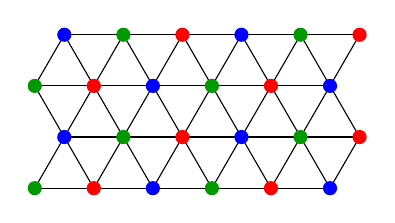
\begin{tikzpicture}[scale=0.75]
  \foreach \j in {0,1,2,3} \draw ({0.5*mod(\j,2)},{0.866*\j}) -- ++(5,0);
  \foreach \i in {0,...,5} {\draw (\i,0) -- ++(60:1) -- ++(120:1) -- ++(60:1);}
  \foreach \i in {1,...,5} {\draw (\i,0) -- ++(120:1) -- ++(60:1) -- ++(120:1);}
  \foreach \j in {0,1,2,3} \foreach \i in {0,...,5} {
    \pgfmathtruncatemacro{\c}{mod(\i-floor(\j/2)-\j+30,3)}
    \pgfmathsetmacro{\xx}{\i+0.5*mod(\j,2)}
    \ifnum\c=0 \fill[green!60!black] (\xx,{0.866*\j}) circle (0.12);\fi
    \ifnum\c=1 \fill[red] (\xx,{0.866*\j}) circle (0.12);\fi
    \ifnum\c=2 \fill[blue] (\xx,{0.866*\j}) circle (0.12);\fi
  }
\end{tikzpicture}
\diagramcaption{One ground state of krypton on graphite, drawn on the dual triangular lattice. Green sites are Kr atoms;
each is surrounded by vacant faces of $\Lambda_{hc}$, i.e.\ vacant sites of $\Lambda_{hc}^* = \Lambda_{tri}$. The three
colors mark the three sublattices of $\Lambda_{tri}$.}
\end{diagram}

The picture shows one ground state of the system, with each Kr atom (indicated by green) surrounded by vacant faces of
$\Lambda_{hc}\leftrightarrow$ vacant sites of $\Lambda_{hc}^* = \Lambda_{tri}$. This is called ``$\frac13$ coverage'', since
$\frac13$ of the faces of $\Lambda_{hc}$ (i.e.\ $\frac13$ of the sites of $\Lambda_{tri}$) are occupied by the Kr atoms. Since
$\Lambda_{tri} = \Lambda_1\oplus\Lambda_2\oplus\Lambda_3$ (green, red and blue sublattices), there are two other equivalent
ground states, where the Kr atoms are adsorbed on the other set of faces of $\Lambda_{hc}$ (graphene surface), i.e.\ the
vertices on the other two sublattices of $\Lambda_{tri}$ (red or blue). This is equivalent to the 3 degenerate ground states
of the $q = 3$ ferromagnetic Potts model with $\sigma_i = 1$, 2, or 3 $\forall\,i$. So this system can be described by this
model.
